\documentclass[twoside]{book}

% Packages required by doxygen
\usepackage{fixltx2e}
\usepackage{calc}
\usepackage{doxygen}
\usepackage[export]{adjustbox} % also loads graphicx
\usepackage{graphicx}
\usepackage[utf8]{inputenc}
\usepackage{makeidx}
\usepackage{multicol}
\usepackage{multirow}
\PassOptionsToPackage{warn}{textcomp}
\usepackage{textcomp}
\usepackage[nointegrals]{wasysym}
\usepackage[table]{xcolor}

% Font selection
\usepackage[T1]{fontenc}
\usepackage[scaled=.90]{helvet}
\usepackage{courier}
\usepackage{amssymb}
\usepackage{sectsty}
\renewcommand{\familydefault}{\sfdefault}
\allsectionsfont{%
  \fontseries{bc}\selectfont%
  \color{darkgray}%
}
\renewcommand{\DoxyLabelFont}{%
  \fontseries{bc}\selectfont%
  \color{darkgray}%
}
\newcommand{\+}{\discretionary{\mbox{\scriptsize$\hookleftarrow$}}{}{}}

% Page & text layout
\usepackage{geometry}
\geometry{%
  a4paper,%
  top=2.5cm,%
  bottom=2.5cm,%
  left=2.5cm,%
  right=2.5cm%
}
\tolerance=750
\hfuzz=15pt
\hbadness=750
\setlength{\emergencystretch}{15pt}
\setlength{\parindent}{0cm}
\setlength{\parskip}{3ex plus 2ex minus 2ex}
\makeatletter
\renewcommand{\paragraph}{%
  \@startsection{paragraph}{4}{0ex}{-1.0ex}{1.0ex}{%
    \normalfont\normalsize\bfseries\SS@parafont%
  }%
}
\renewcommand{\subparagraph}{%
  \@startsection{subparagraph}{5}{0ex}{-1.0ex}{1.0ex}{%
    \normalfont\normalsize\bfseries\SS@subparafont%
  }%
}
\makeatother

% Headers & footers
\usepackage{fancyhdr}
\pagestyle{fancyplain}
\fancyhead[LE]{\fancyplain{}{\bfseries\thepage}}
\fancyhead[CE]{\fancyplain{}{}}
\fancyhead[RE]{\fancyplain{}{\bfseries\leftmark}}
\fancyhead[LO]{\fancyplain{}{\bfseries\rightmark}}
\fancyhead[CO]{\fancyplain{}{}}
\fancyhead[RO]{\fancyplain{}{\bfseries\thepage}}
\fancyfoot[LE]{\fancyplain{}{}}
\fancyfoot[CE]{\fancyplain{}{}}
\fancyfoot[RE]{\fancyplain{}{\bfseries\scriptsize Generated by Doxygen }}
\fancyfoot[LO]{\fancyplain{}{\bfseries\scriptsize Generated by Doxygen }}
\fancyfoot[CO]{\fancyplain{}{}}
\fancyfoot[RO]{\fancyplain{}{}}
\renewcommand{\footrulewidth}{0.4pt}
\renewcommand{\chaptermark}[1]{%
  \markboth{#1}{}%
}
\renewcommand{\sectionmark}[1]{%
  \markright{\thesection\ #1}%
}

% Indices & bibliography
\usepackage{natbib}
\usepackage[titles]{tocloft}
\setcounter{tocdepth}{3}
\setcounter{secnumdepth}{5}
\makeindex

% Hyperlinks (required, but should be loaded last)
\usepackage{ifpdf}
\ifpdf
  \usepackage[pdftex,pagebackref=true]{hyperref}
\else
  \usepackage[ps2pdf,pagebackref=true]{hyperref}
\fi
\hypersetup{%
  colorlinks=true,%
  linkcolor=blue,%
  citecolor=blue,%
  unicode%
}

% Custom commands
\newcommand{\clearemptydoublepage}{%
  \newpage{\pagestyle{empty}\cleardoublepage}%
}

\usepackage{caption}
\captionsetup{labelsep=space,justification=centering,font={bf},singlelinecheck=off,skip=4pt,position=top}

%===== C O N T E N T S =====

\begin{document}

% Titlepage & ToC
\hypersetup{pageanchor=false,
             bookmarksnumbered=true,
             pdfencoding=unicode
            }
\pagenumbering{alph}
\begin{titlepage}
\vspace*{7cm}
\begin{center}%
{\Large Calculator \\[1ex]\large 1.\+0 }\\
\vspace*{1cm}
{\large Generated by Doxygen 1.8.13}\\
\end{center}
\end{titlepage}
\clearemptydoublepage
\pagenumbering{roman}
\tableofcontents
\clearemptydoublepage
\pagenumbering{arabic}
\hypersetup{pageanchor=true}

%--- Begin generated contents ---
\chapter{Documentation for team school project.}
\label{index}\hypertarget{index}{}\hypertarget{index_intro_sec}{}\section{Introduction}\label{index_intro_sec}
Hello!

On this page you can see everything about our school project. Search in namespaces, classes or files to find more.\hypertarget{index_authors_sec}{}\section{Authors}\label{index_authors_sec}
xjurke02 Jurkechová Adriana

xstefe11 Štefeková Nina

xsveck00 Švecková Sabína

xvanop01 Vaňo Peter\hypertarget{index_school_sec}{}\section{Brno University of Technology F\+IT}\label{index_school_sec}
We are from Faculty of Information Technology. For more information about our university visit\+:

\href{https://www.fit.vut.cz/.en}{\tt Faculty of Information Technology B\+UT}

\href{https://www.vutbr.cz/en/}{\tt Brno University of Technology} 
\chapter{Namespace Index}
\section{Namespace List}
Here is a list of all namespaces with brief descriptions\+:\begin{DoxyCompactList}
\item\contentsline{section}{\hyperlink{namespaceDanaProfessional}{Dana\+Professional} }{\pageref{namespaceDanaProfessional}}{}
\item\contentsline{section}{\hyperlink{namespaceDanaSimple}{Dana\+Simple} }{\pageref{namespaceDanaSimple}}{}
\item\contentsline{section}{\hyperlink{namespaceMathLibraryTest}{Math\+Library\+Test} }{\pageref{namespaceMathLibraryTest}}{}
\item\contentsline{section}{\hyperlink{namespacepokus}{pokus} }{\pageref{namespacepokus}}{}
\item\contentsline{section}{\hyperlink{namespacepokus_1_1Properties}{pokus.\+Properties} }{\pageref{namespacepokus_1_1Properties}}{}
\item\contentsline{section}{\hyperlink{namespaceProfiler}{Profiler} }{\pageref{namespaceProfiler}}{}
\end{DoxyCompactList}

\chapter{Hierarchical Index}
\section{Class Hierarchy}
This inheritance list is sorted roughly, but not completely, alphabetically\+:\begin{DoxyCompactList}
\item \contentsline{section}{Math\+Library\+Test.\+Dana\+Professional}{\pageref{classMathLibraryTest_1_1DanaProfessional}}{}
\item \contentsline{section}{Math\+Library\+Test.\+Dana\+Simple\+Test}{\pageref{classMathLibraryTest_1_1DanaSimpleTest}}{}
\item Form\begin{DoxyCompactList}
\item \contentsline{section}{pokus.\+Form1}{\pageref{classpokus_1_1Form1}}{}
\end{DoxyCompactList}
\item \contentsline{section}{Dana\+Professional.\+Operations\+Professional}{\pageref{classDanaProfessional_1_1OperationsProfessional}}{}
\item \contentsline{section}{Dana\+Simple.\+Operations\+Simple}{\pageref{classDanaSimple_1_1OperationsSimple}}{}
\item \contentsline{section}{Profiler.\+Profiler}{\pageref{classProfiler_1_1Profiler}}{}
\item \contentsline{section}{Profiler.\+Profiler\+Counters}{\pageref{classProfiler_1_1ProfilerCounters}}{}
\item \contentsline{section}{pokus.\+Program}{\pageref{classpokus_1_1Program}}{}
\item \contentsline{section}{Profiler.\+Suma}{\pageref{classProfiler_1_1Suma}}{}
\end{DoxyCompactList}

\chapter{Class Index}
\section{Class List}
Here are the classes, structs, unions and interfaces with brief descriptions\+:\begin{DoxyCompactList}
\item\contentsline{section}{\hyperlink{classMathLibraryTest_1_1DanaProfessional}{Math\+Library\+Test.\+Dana\+Professional} \\*Operations\+Professional tests }{\pageref{classMathLibraryTest_1_1DanaProfessional}}{}
\item\contentsline{section}{\hyperlink{classMathLibraryTest_1_1DanaSimpleTest}{Math\+Library\+Test.\+Dana\+Simple\+Test} \\*Operations\+Simple tests }{\pageref{classMathLibraryTest_1_1DanaSimpleTest}}{}
\item\contentsline{section}{\hyperlink{classpokus_1_1Form1}{pokus.\+Form1} }{\pageref{classpokus_1_1Form1}}{}
\item\contentsline{section}{\hyperlink{classDanaProfessional_1_1OperationsProfessional}{Dana\+Professional.\+Operations\+Professional} \\*Extended Math library class }{\pageref{classDanaProfessional_1_1OperationsProfessional}}{}
\item\contentsline{section}{\hyperlink{classDanaSimple_1_1OperationsSimple}{Dana\+Simple.\+Operations\+Simple} \\*Simple Math library class }{\pageref{classDanaSimple_1_1OperationsSimple}}{}
\item\contentsline{section}{\hyperlink{classProfiler_1_1Profiler}{Profiler.\+Profiler} \\*Executable }{\pageref{classProfiler_1_1Profiler}}{}
\item\contentsline{section}{\hyperlink{classProfiler_1_1ProfilerCounters}{Profiler.\+Profiler\+Counters} \\*\hyperlink{classProfiler_1_1Profiler}{Profiler} handler }{\pageref{classProfiler_1_1ProfilerCounters}}{}
\item\contentsline{section}{\hyperlink{classpokus_1_1Program}{pokus.\+Program} }{\pageref{classpokus_1_1Program}}{}
\item\contentsline{section}{\hyperlink{classProfiler_1_1Suma}{Profiler.\+Suma} \\*Sum handler }{\pageref{classProfiler_1_1Suma}}{}
\end{DoxyCompactList}

\chapter{File Index}
\section{File List}
Here is a list of all files with brief descriptions\+:\begin{DoxyCompactList}
\item\contentsline{section}{\hyperlink{Form1_8cs}{Form1.\+cs} }{\pageref{Form1_8cs}}{}
\item\contentsline{section}{\hyperlink{Form1_8Designer_8cs}{Form1.\+Designer.\+cs} }{\pageref{Form1_8Designer_8cs}}{}
\item\contentsline{section}{\hyperlink{Program_8cs}{Program.\+cs} }{\pageref{Program_8cs}}{}
\item\contentsline{section}{math\+\_\+library/math\+\_\+library/\hyperlink{dana__professional_8cs}{dana\+\_\+professional.\+cs} \\*Extended Math library }{\pageref{dana__professional_8cs}}{}
\item\contentsline{section}{math\+\_\+library/math\+\_\+library/\hyperlink{dana__simple_8cs}{dana\+\_\+simple.\+cs} \\*Math library }{\pageref{dana__simple_8cs}}{}
\item\contentsline{section}{math\+\_\+library/math\+\_\+library/obj/\+Debug/netstandard2.\+0/\hyperlink{math__library_2math__library_2obj_2Debug_2netstandard2_80_2math__library_8AssemblyInfo_8cs}{math\+\_\+library.\+Assembly\+Info.\+cs} }{\pageref{math__library_2math__library_2obj_2Debug_2netstandard2_80_2math__library_8AssemblyInfo_8cs}}{}
\item\contentsline{section}{math\+\_\+library/math\+\_\+library/obj/\+Release/netstandard2.\+0/\hyperlink{math__library_2math__library_2obj_2Release_2netstandard2_80_2math__library_8AssemblyInfo_8cs}{math\+\_\+library.\+Assembly\+Info.\+cs} }{\pageref{math__library_2math__library_2obj_2Release_2netstandard2_80_2math__library_8AssemblyInfo_8cs}}{}
\item\contentsline{section}{math\+\_\+library/\+Math\+Library\+Test/\hyperlink{test__dana_8cs}{test\+\_\+dana.\+cs} \\*Tests for Math library }{\pageref{test__dana_8cs}}{}
\item\contentsline{section}{math\+\_\+library/\+Math\+Library\+Test/obj/\+Debug/netcoreapp3.\+1/\hyperlink{Debug_2netcoreapp3_81_2MathLibraryTest_8AssemblyInfo_8cs}{Math\+Library\+Test.\+Assembly\+Info.\+cs} }{\pageref{Debug_2netcoreapp3_81_2MathLibraryTest_8AssemblyInfo_8cs}}{}
\item\contentsline{section}{math\+\_\+library/\+Math\+Library\+Test/obj/\+Release/netcoreapp3.\+1/\hyperlink{Release_2netcoreapp3_81_2MathLibraryTest_8AssemblyInfo_8cs}{Math\+Library\+Test.\+Assembly\+Info.\+cs} }{\pageref{Release_2netcoreapp3_81_2MathLibraryTest_8AssemblyInfo_8cs}}{}
\item\contentsline{section}{math\+\_\+library/\+Profiler/\hyperlink{Profiler_8cs}{Profiler.\+cs} }{\pageref{Profiler_8cs}}{}
\item\contentsline{section}{math\+\_\+library/\+Profiler/obj/\+Debug/netcoreapp3.\+1/\hyperlink{Debug_2netcoreapp3_81_2Profiler_8AssemblyInfo_8cs}{Profiler.\+Assembly\+Info.\+cs} }{\pageref{Debug_2netcoreapp3_81_2Profiler_8AssemblyInfo_8cs}}{}
\item\contentsline{section}{math\+\_\+library/\+Profiler/obj/\+Release/netcoreapp3.\+1/\hyperlink{Release_2netcoreapp3_81_2Profiler_8AssemblyInfo_8cs}{Profiler.\+Assembly\+Info.\+cs} }{\pageref{Release_2netcoreapp3_81_2Profiler_8AssemblyInfo_8cs}}{}
\item\contentsline{section}{obj/\+Debug/netstandard2.\+0/\hyperlink{math__library_01_072_08_8AssemblyInfo_8cs}{math\+\_\+library (2).\+Assembly\+Info.\+cs} }{\pageref{math__library_01_072_08_8AssemblyInfo_8cs}}{}
\item\contentsline{section}{obj/\+Debug/netstandard2.\+0/\hyperlink{obj_2Debug_2netstandard2_80_2math__library_8AssemblyInfo_8cs}{math\+\_\+library.\+Assembly\+Info.\+cs} }{\pageref{obj_2Debug_2netstandard2_80_2math__library_8AssemblyInfo_8cs}}{}
\item\contentsline{section}{Properties/\hyperlink{AssemblyInfo_8cs}{Assembly\+Info.\+cs} }{\pageref{AssemblyInfo_8cs}}{}
\item\contentsline{section}{Properties/\hyperlink{Resources_8Designer_8cs}{Resources.\+Designer.\+cs} }{\pageref{Resources_8Designer_8cs}}{}
\item\contentsline{section}{Properties/\hyperlink{Settings_8Designer_8cs}{Settings.\+Designer.\+cs} }{\pageref{Settings_8Designer_8cs}}{}
\end{DoxyCompactList}

\chapter{Namespace Documentation}
\hypertarget{namespaceDanaProfessional}{}\section{Dana\+Professional Namespace Reference}
\label{namespaceDanaProfessional}\index{Dana\+Professional@{Dana\+Professional}}
\subsection*{Classes}
\begin{DoxyCompactItemize}
\item 
class \hyperlink{classDanaProfessional_1_1OperationsProfessional}{Operations\+Professional}
\begin{DoxyCompactList}\small\item\em Extended Math library class. \end{DoxyCompactList}\end{DoxyCompactItemize}

\hypertarget{namespaceDanaSimple}{}\section{Dana\+Simple Namespace Reference}
\label{namespaceDanaSimple}\index{Dana\+Simple@{Dana\+Simple}}
\subsection*{Classes}
\begin{DoxyCompactItemize}
\item 
class \hyperlink{classDanaSimple_1_1OperationsSimple}{Operations\+Simple}
\begin{DoxyCompactList}\small\item\em Simple Math library class. \end{DoxyCompactList}\end{DoxyCompactItemize}

\hypertarget{namespaceMathLibraryTest}{}\section{Math\+Library\+Test Namespace Reference}
\label{namespaceMathLibraryTest}\index{Math\+Library\+Test@{Math\+Library\+Test}}
\subsection*{Classes}
\begin{DoxyCompactItemize}
\item 
class \hyperlink{classMathLibraryTest_1_1DanaProfessional}{Dana\+Professional}
\begin{DoxyCompactList}\small\item\em Operations\+Professional tests. \end{DoxyCompactList}\item 
class \hyperlink{classMathLibraryTest_1_1DanaSimpleTest}{Dana\+Simple\+Test}
\begin{DoxyCompactList}\small\item\em Operations\+Simple tests. \end{DoxyCompactList}\end{DoxyCompactItemize}

\hypertarget{namespacepokus}{}\section{pokus Namespace Reference}
\label{namespacepokus}\index{pokus@{pokus}}
\subsection*{Namespaces}
\begin{DoxyCompactItemize}
\item 
namespace \hyperlink{namespacepokus_1_1Properties}{Properties}
\end{DoxyCompactItemize}
\subsection*{Classes}
\begin{DoxyCompactItemize}
\item 
class \hyperlink{classpokus_1_1Form1}{Form1}
\item 
class \hyperlink{classpokus_1_1Program}{Program}
\end{DoxyCompactItemize}

\hypertarget{namespacepokus_1_1Properties}{}\section{pokus.\+Properties Namespace Reference}
\label{namespacepokus_1_1Properties}\index{pokus.\+Properties@{pokus.\+Properties}}
\subsection*{Classes}
\begin{DoxyCompactItemize}
\item 
class {\bfseries Resources}
\begin{DoxyCompactList}\small\item\em A strongly-\/typed resource class, for looking up localized strings, etc. \end{DoxyCompactList}\item 
class {\bfseries Settings}
\end{DoxyCompactItemize}

\hypertarget{namespaceProfiler}{}\section{Profiler Namespace Reference}
\label{namespaceProfiler}\index{Profiler@{Profiler}}
\subsection*{Classes}
\begin{DoxyCompactItemize}
\item 
class \hyperlink{classProfiler_1_1Profiler}{Profiler}
\begin{DoxyCompactList}\small\item\em Executable. \end{DoxyCompactList}\item 
class \hyperlink{classProfiler_1_1ProfilerCounters}{Profiler\+Counters}
\begin{DoxyCompactList}\small\item\em \hyperlink{classProfiler_1_1Profiler}{Profiler} handler. \end{DoxyCompactList}\item 
class \hyperlink{classProfiler_1_1Suma}{Suma}
\begin{DoxyCompactList}\small\item\em Sum handler. \end{DoxyCompactList}\end{DoxyCompactItemize}

\chapter{Class Documentation}
\hypertarget{classMathLibraryTest_1_1DanaProfessional}{}\section{Math\+Library\+Test.\+Dana\+Professional Class Reference}
\label{classMathLibraryTest_1_1DanaProfessional}\index{Math\+Library\+Test.\+Dana\+Professional@{Math\+Library\+Test.\+Dana\+Professional}}


Operations\+Professional tests.  


\subsection*{Public Member Functions}
\begin{DoxyCompactItemize}
\item 
void \hyperlink{classMathLibraryTest_1_1DanaProfessional_a57932b88ac96d31c774b02fe1c23c8ee}{Test\+Exp} ()
\begin{DoxyCompactList}\small\item\em Operations\+Professional.\+Exp tests. \end{DoxyCompactList}\item 
void \hyperlink{classMathLibraryTest_1_1DanaProfessional_a7ab9375202b08f4990dbd7f97fb9ba54}{Test\+Rt} ()
\begin{DoxyCompactList}\small\item\em Operations\+Professional.\+Rt tests. \end{DoxyCompactList}\item 
void \hyperlink{classMathLibraryTest_1_1DanaProfessional_a21d72d33ba0efcbbe8b693075630ac6f}{Test\+Abs} ()
\begin{DoxyCompactList}\small\item\em Operations\+Professional.\+Abs tests. \end{DoxyCompactList}\end{DoxyCompactItemize}


\subsection{Detailed Description}
Operations\+Professional tests. 

\subsection{Member Function Documentation}
\mbox{\Hypertarget{classMathLibraryTest_1_1DanaProfessional_a21d72d33ba0efcbbe8b693075630ac6f}\label{classMathLibraryTest_1_1DanaProfessional_a21d72d33ba0efcbbe8b693075630ac6f}} 
\index{Math\+Library\+Test\+::\+Dana\+Professional@{Math\+Library\+Test\+::\+Dana\+Professional}!Test\+Abs@{Test\+Abs}}
\index{Test\+Abs@{Test\+Abs}!Math\+Library\+Test\+::\+Dana\+Professional@{Math\+Library\+Test\+::\+Dana\+Professional}}
\subsubsection{\texorpdfstring{Test\+Abs()}{TestAbs()}}
{\footnotesize\ttfamily void Math\+Library\+Test.\+Dana\+Professional.\+Test\+Abs (\begin{DoxyParamCaption}{ }\end{DoxyParamCaption})\hspace{0.3cm}{\ttfamily [inline]}}



Operations\+Professional.\+Abs tests. 

\mbox{\Hypertarget{classMathLibraryTest_1_1DanaProfessional_a57932b88ac96d31c774b02fe1c23c8ee}\label{classMathLibraryTest_1_1DanaProfessional_a57932b88ac96d31c774b02fe1c23c8ee}} 
\index{Math\+Library\+Test\+::\+Dana\+Professional@{Math\+Library\+Test\+::\+Dana\+Professional}!Test\+Exp@{Test\+Exp}}
\index{Test\+Exp@{Test\+Exp}!Math\+Library\+Test\+::\+Dana\+Professional@{Math\+Library\+Test\+::\+Dana\+Professional}}
\subsubsection{\texorpdfstring{Test\+Exp()}{TestExp()}}
{\footnotesize\ttfamily void Math\+Library\+Test.\+Dana\+Professional.\+Test\+Exp (\begin{DoxyParamCaption}{ }\end{DoxyParamCaption})\hspace{0.3cm}{\ttfamily [inline]}}



Operations\+Professional.\+Exp tests. 

\mbox{\Hypertarget{classMathLibraryTest_1_1DanaProfessional_a7ab9375202b08f4990dbd7f97fb9ba54}\label{classMathLibraryTest_1_1DanaProfessional_a7ab9375202b08f4990dbd7f97fb9ba54}} 
\index{Math\+Library\+Test\+::\+Dana\+Professional@{Math\+Library\+Test\+::\+Dana\+Professional}!Test\+Rt@{Test\+Rt}}
\index{Test\+Rt@{Test\+Rt}!Math\+Library\+Test\+::\+Dana\+Professional@{Math\+Library\+Test\+::\+Dana\+Professional}}
\subsubsection{\texorpdfstring{Test\+Rt()}{TestRt()}}
{\footnotesize\ttfamily void Math\+Library\+Test.\+Dana\+Professional.\+Test\+Rt (\begin{DoxyParamCaption}{ }\end{DoxyParamCaption})\hspace{0.3cm}{\ttfamily [inline]}}



Operations\+Professional.\+Rt tests. 



The documentation for this class was generated from the following file\+:\begin{DoxyCompactItemize}
\item 
math\+\_\+library/\+Math\+Library\+Test/\hyperlink{test__dana_8cs}{test\+\_\+dana.\+cs}\end{DoxyCompactItemize}

\hypertarget{classMathLibraryTest_1_1DanaSimpleTest}{}\section{Math\+Library\+Test.\+Dana\+Simple\+Test Class Reference}
\label{classMathLibraryTest_1_1DanaSimpleTest}\index{Math\+Library\+Test.\+Dana\+Simple\+Test@{Math\+Library\+Test.\+Dana\+Simple\+Test}}


Operations\+Simple tests.  


\subsection*{Public Member Functions}
\begin{DoxyCompactItemize}
\item 
void \hyperlink{classMathLibraryTest_1_1DanaSimpleTest_af9f0ba76d61b68ef4bc165818530c3a0}{Test\+Plus} ()
\begin{DoxyCompactList}\small\item\em Operations\+Simple.\+Plus tests. \end{DoxyCompactList}\item 
void \hyperlink{classMathLibraryTest_1_1DanaSimpleTest_adbd49d0988fdaa66142f38d73238a784}{Test\+Minus} ()
\begin{DoxyCompactList}\small\item\em Operations\+Simple.\+Minus tests. \end{DoxyCompactList}\item 
void \hyperlink{classMathLibraryTest_1_1DanaSimpleTest_ad304d5b8df0f62bef4d3f12ae8dfdb37}{Test\+Multi} ()
\begin{DoxyCompactList}\small\item\em Operations\+Simple.\+Multi tests. \end{DoxyCompactList}\item 
void \hyperlink{classMathLibraryTest_1_1DanaSimpleTest_a2db7ba0f1dd7665624c1eeecba0000ea}{Test\+Div} ()
\begin{DoxyCompactList}\small\item\em Operations\+Simple.\+Div tests. \end{DoxyCompactList}\item 
void \hyperlink{classMathLibraryTest_1_1DanaSimpleTest_a8bc466c1cfe224c7857ef7442c19105c}{Test\+Factorial} ()
\begin{DoxyCompactList}\small\item\em Operations\+Simple.\+Factorial tests. \end{DoxyCompactList}\end{DoxyCompactItemize}


\subsection{Detailed Description}
Operations\+Simple tests. 

\subsection{Member Function Documentation}
\mbox{\Hypertarget{classMathLibraryTest_1_1DanaSimpleTest_a2db7ba0f1dd7665624c1eeecba0000ea}\label{classMathLibraryTest_1_1DanaSimpleTest_a2db7ba0f1dd7665624c1eeecba0000ea}} 
\index{Math\+Library\+Test\+::\+Dana\+Simple\+Test@{Math\+Library\+Test\+::\+Dana\+Simple\+Test}!Test\+Div@{Test\+Div}}
\index{Test\+Div@{Test\+Div}!Math\+Library\+Test\+::\+Dana\+Simple\+Test@{Math\+Library\+Test\+::\+Dana\+Simple\+Test}}
\subsubsection{\texorpdfstring{Test\+Div()}{TestDiv()}}
{\footnotesize\ttfamily void Math\+Library\+Test.\+Dana\+Simple\+Test.\+Test\+Div (\begin{DoxyParamCaption}{ }\end{DoxyParamCaption})\hspace{0.3cm}{\ttfamily [inline]}}



Operations\+Simple.\+Div tests. 

\mbox{\Hypertarget{classMathLibraryTest_1_1DanaSimpleTest_a8bc466c1cfe224c7857ef7442c19105c}\label{classMathLibraryTest_1_1DanaSimpleTest_a8bc466c1cfe224c7857ef7442c19105c}} 
\index{Math\+Library\+Test\+::\+Dana\+Simple\+Test@{Math\+Library\+Test\+::\+Dana\+Simple\+Test}!Test\+Factorial@{Test\+Factorial}}
\index{Test\+Factorial@{Test\+Factorial}!Math\+Library\+Test\+::\+Dana\+Simple\+Test@{Math\+Library\+Test\+::\+Dana\+Simple\+Test}}
\subsubsection{\texorpdfstring{Test\+Factorial()}{TestFactorial()}}
{\footnotesize\ttfamily void Math\+Library\+Test.\+Dana\+Simple\+Test.\+Test\+Factorial (\begin{DoxyParamCaption}{ }\end{DoxyParamCaption})\hspace{0.3cm}{\ttfamily [inline]}}



Operations\+Simple.\+Factorial tests. 

\mbox{\Hypertarget{classMathLibraryTest_1_1DanaSimpleTest_adbd49d0988fdaa66142f38d73238a784}\label{classMathLibraryTest_1_1DanaSimpleTest_adbd49d0988fdaa66142f38d73238a784}} 
\index{Math\+Library\+Test\+::\+Dana\+Simple\+Test@{Math\+Library\+Test\+::\+Dana\+Simple\+Test}!Test\+Minus@{Test\+Minus}}
\index{Test\+Minus@{Test\+Minus}!Math\+Library\+Test\+::\+Dana\+Simple\+Test@{Math\+Library\+Test\+::\+Dana\+Simple\+Test}}
\subsubsection{\texorpdfstring{Test\+Minus()}{TestMinus()}}
{\footnotesize\ttfamily void Math\+Library\+Test.\+Dana\+Simple\+Test.\+Test\+Minus (\begin{DoxyParamCaption}{ }\end{DoxyParamCaption})\hspace{0.3cm}{\ttfamily [inline]}}



Operations\+Simple.\+Minus tests. 

\mbox{\Hypertarget{classMathLibraryTest_1_1DanaSimpleTest_ad304d5b8df0f62bef4d3f12ae8dfdb37}\label{classMathLibraryTest_1_1DanaSimpleTest_ad304d5b8df0f62bef4d3f12ae8dfdb37}} 
\index{Math\+Library\+Test\+::\+Dana\+Simple\+Test@{Math\+Library\+Test\+::\+Dana\+Simple\+Test}!Test\+Multi@{Test\+Multi}}
\index{Test\+Multi@{Test\+Multi}!Math\+Library\+Test\+::\+Dana\+Simple\+Test@{Math\+Library\+Test\+::\+Dana\+Simple\+Test}}
\subsubsection{\texorpdfstring{Test\+Multi()}{TestMulti()}}
{\footnotesize\ttfamily void Math\+Library\+Test.\+Dana\+Simple\+Test.\+Test\+Multi (\begin{DoxyParamCaption}{ }\end{DoxyParamCaption})\hspace{0.3cm}{\ttfamily [inline]}}



Operations\+Simple.\+Multi tests. 

\mbox{\Hypertarget{classMathLibraryTest_1_1DanaSimpleTest_af9f0ba76d61b68ef4bc165818530c3a0}\label{classMathLibraryTest_1_1DanaSimpleTest_af9f0ba76d61b68ef4bc165818530c3a0}} 
\index{Math\+Library\+Test\+::\+Dana\+Simple\+Test@{Math\+Library\+Test\+::\+Dana\+Simple\+Test}!Test\+Plus@{Test\+Plus}}
\index{Test\+Plus@{Test\+Plus}!Math\+Library\+Test\+::\+Dana\+Simple\+Test@{Math\+Library\+Test\+::\+Dana\+Simple\+Test}}
\subsubsection{\texorpdfstring{Test\+Plus()}{TestPlus()}}
{\footnotesize\ttfamily void Math\+Library\+Test.\+Dana\+Simple\+Test.\+Test\+Plus (\begin{DoxyParamCaption}{ }\end{DoxyParamCaption})\hspace{0.3cm}{\ttfamily [inline]}}



Operations\+Simple.\+Plus tests. 



The documentation for this class was generated from the following file\+:\begin{DoxyCompactItemize}
\item 
math\+\_\+library/\+Math\+Library\+Test/\hyperlink{test__dana_8cs}{test\+\_\+dana.\+cs}\end{DoxyCompactItemize}

\hypertarget{classpokus_1_1Form1}{}\section{pokus.\+Form1 Class Reference}
\label{classpokus_1_1Form1}\index{pokus.\+Form1@{pokus.\+Form1}}
Inheritance diagram for pokus.\+Form1\+:\begin{figure}[H]
\begin{center}
\leavevmode
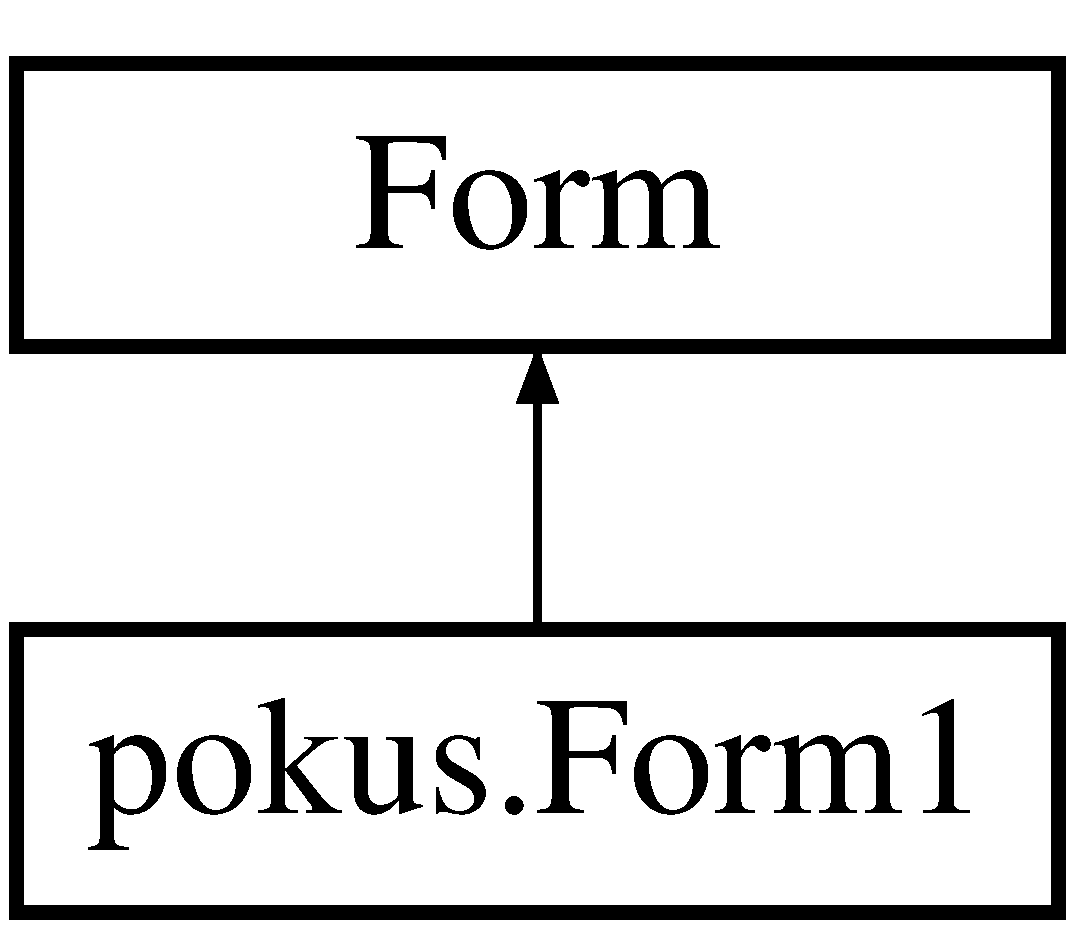
\includegraphics[height=2.000000cm]{classpokus_1_1Form1}
\end{center}
\end{figure}
\subsection*{Public Member Functions}
\begin{DoxyCompactItemize}
\item 
\hyperlink{classpokus_1_1Form1_ab64d54a396652470204211a4be1e404a}{Form1} ()
\end{DoxyCompactItemize}
\subsection*{Public Attributes}
\begin{DoxyCompactItemize}
\item 
System.\+Windows.\+Forms.\+Button \hyperlink{classpokus_1_1Form1_a4f9f5e2ad5a81fd690dae321c822e9d6}{button3}
\item 
System.\+Windows.\+Forms.\+Button \hyperlink{classpokus_1_1Form1_a0176e28b0300cffaf5233221160d8819}{button6}
\item 
System.\+Windows.\+Forms.\+Button \hyperlink{classpokus_1_1Form1_a8c13359112a696acc4115dabbbf6384a}{buttonequals}
\item 
System.\+Windows.\+Forms.\+Button \hyperlink{classpokus_1_1Form1_a8a4e01d4f371e552e2992b3fce4f0caf}{buttondiv}
\item 
System.\+Windows.\+Forms.\+Button \hyperlink{classpokus_1_1Form1_a967f22539b61592f15df2ae6a087b6e5}{buttonplus}
\item 
System.\+Windows.\+Forms.\+Button \hyperlink{classpokus_1_1Form1_a192b6a454ea0c3b9c2472b55301ad3e9}{buttonsub}
\item 
System.\+Windows.\+Forms.\+Button \hyperlink{classpokus_1_1Form1_a9c09c5cca3e7ea82d087747de71a3466}{buttonmul}
\item 
System.\+Windows.\+Forms.\+Button \hyperlink{classpokus_1_1Form1_a627ac5a2200ea94b232a465ccf7ad883}{buttonpower}
\item 
System.\+Windows.\+Forms.\+Button \hyperlink{classpokus_1_1Form1_a1b0a460ccc81b4eb38a892d0587434a9}{buttonfact}
\item 
System.\+Windows.\+Forms.\+Button \hyperlink{classpokus_1_1Form1_a4f6946b9f61cef4dfc810e4336b51348}{buttonabs}
\item 
System.\+Windows.\+Forms.\+Button \hyperlink{classpokus_1_1Form1_a11a1d9f87f27db44987024bfe4c41912}{buttonce}
\item 
System.\+Windows.\+Forms.\+Button \hyperlink{classpokus_1_1Form1_adb3eefca0a1ebdaad882b13e3f1f5ff3}{button11}
\item 
System.\+Windows.\+Forms.\+Button \hyperlink{classpokus_1_1Form1_a7717a2a50c484f641bdcc54cd679a193}{root}
\end{DoxyCompactItemize}
\subsection*{Protected Member Functions}
\begin{DoxyCompactItemize}
\item 
override void \hyperlink{classpokus_1_1Form1_a24b23515810a6e52f80e600649e7f5a3}{Dispose} (bool disposing)
\begin{DoxyCompactList}\small\item\em Clean up any resources being used. \end{DoxyCompactList}\end{DoxyCompactItemize}


\subsection{Constructor \& Destructor Documentation}
\mbox{\Hypertarget{classpokus_1_1Form1_ab64d54a396652470204211a4be1e404a}\label{classpokus_1_1Form1_ab64d54a396652470204211a4be1e404a}} 
\index{pokus\+::\+Form1@{pokus\+::\+Form1}!Form1@{Form1}}
\index{Form1@{Form1}!pokus\+::\+Form1@{pokus\+::\+Form1}}
\subsubsection{\texorpdfstring{Form1()}{Form1()}}
{\footnotesize\ttfamily pokus.\+Form1.\+Form1 (\begin{DoxyParamCaption}{ }\end{DoxyParamCaption})\hspace{0.3cm}{\ttfamily [inline]}}



\subsection{Member Function Documentation}
\mbox{\Hypertarget{classpokus_1_1Form1_a24b23515810a6e52f80e600649e7f5a3}\label{classpokus_1_1Form1_a24b23515810a6e52f80e600649e7f5a3}} 
\index{pokus\+::\+Form1@{pokus\+::\+Form1}!Dispose@{Dispose}}
\index{Dispose@{Dispose}!pokus\+::\+Form1@{pokus\+::\+Form1}}
\subsubsection{\texorpdfstring{Dispose()}{Dispose()}}
{\footnotesize\ttfamily override void pokus.\+Form1.\+Dispose (\begin{DoxyParamCaption}\item[{bool}]{disposing }\end{DoxyParamCaption})\hspace{0.3cm}{\ttfamily [inline]}, {\ttfamily [protected]}}



Clean up any resources being used. 


\begin{DoxyParams}{Parameters}
{\em disposing} & true if managed resources should be disposed; otherwise, false.\\
\hline
\end{DoxyParams}


\subsection{Member Data Documentation}
\mbox{\Hypertarget{classpokus_1_1Form1_adb3eefca0a1ebdaad882b13e3f1f5ff3}\label{classpokus_1_1Form1_adb3eefca0a1ebdaad882b13e3f1f5ff3}} 
\index{pokus\+::\+Form1@{pokus\+::\+Form1}!button11@{button11}}
\index{button11@{button11}!pokus\+::\+Form1@{pokus\+::\+Form1}}
\subsubsection{\texorpdfstring{button11}{button11}}
{\footnotesize\ttfamily System.\+Windows.\+Forms.\+Button pokus.\+Form1.\+button11}

\mbox{\Hypertarget{classpokus_1_1Form1_a4f9f5e2ad5a81fd690dae321c822e9d6}\label{classpokus_1_1Form1_a4f9f5e2ad5a81fd690dae321c822e9d6}} 
\index{pokus\+::\+Form1@{pokus\+::\+Form1}!button3@{button3}}
\index{button3@{button3}!pokus\+::\+Form1@{pokus\+::\+Form1}}
\subsubsection{\texorpdfstring{button3}{button3}}
{\footnotesize\ttfamily System.\+Windows.\+Forms.\+Button pokus.\+Form1.\+button3}

\mbox{\Hypertarget{classpokus_1_1Form1_a0176e28b0300cffaf5233221160d8819}\label{classpokus_1_1Form1_a0176e28b0300cffaf5233221160d8819}} 
\index{pokus\+::\+Form1@{pokus\+::\+Form1}!button6@{button6}}
\index{button6@{button6}!pokus\+::\+Form1@{pokus\+::\+Form1}}
\subsubsection{\texorpdfstring{button6}{button6}}
{\footnotesize\ttfamily System.\+Windows.\+Forms.\+Button pokus.\+Form1.\+button6}

\mbox{\Hypertarget{classpokus_1_1Form1_a4f6946b9f61cef4dfc810e4336b51348}\label{classpokus_1_1Form1_a4f6946b9f61cef4dfc810e4336b51348}} 
\index{pokus\+::\+Form1@{pokus\+::\+Form1}!buttonabs@{buttonabs}}
\index{buttonabs@{buttonabs}!pokus\+::\+Form1@{pokus\+::\+Form1}}
\subsubsection{\texorpdfstring{buttonabs}{buttonabs}}
{\footnotesize\ttfamily System.\+Windows.\+Forms.\+Button pokus.\+Form1.\+buttonabs}

\mbox{\Hypertarget{classpokus_1_1Form1_a11a1d9f87f27db44987024bfe4c41912}\label{classpokus_1_1Form1_a11a1d9f87f27db44987024bfe4c41912}} 
\index{pokus\+::\+Form1@{pokus\+::\+Form1}!buttonce@{buttonce}}
\index{buttonce@{buttonce}!pokus\+::\+Form1@{pokus\+::\+Form1}}
\subsubsection{\texorpdfstring{buttonce}{buttonce}}
{\footnotesize\ttfamily System.\+Windows.\+Forms.\+Button pokus.\+Form1.\+buttonce}

\mbox{\Hypertarget{classpokus_1_1Form1_a8a4e01d4f371e552e2992b3fce4f0caf}\label{classpokus_1_1Form1_a8a4e01d4f371e552e2992b3fce4f0caf}} 
\index{pokus\+::\+Form1@{pokus\+::\+Form1}!buttondiv@{buttondiv}}
\index{buttondiv@{buttondiv}!pokus\+::\+Form1@{pokus\+::\+Form1}}
\subsubsection{\texorpdfstring{buttondiv}{buttondiv}}
{\footnotesize\ttfamily System.\+Windows.\+Forms.\+Button pokus.\+Form1.\+buttondiv}

\mbox{\Hypertarget{classpokus_1_1Form1_a8c13359112a696acc4115dabbbf6384a}\label{classpokus_1_1Form1_a8c13359112a696acc4115dabbbf6384a}} 
\index{pokus\+::\+Form1@{pokus\+::\+Form1}!buttonequals@{buttonequals}}
\index{buttonequals@{buttonequals}!pokus\+::\+Form1@{pokus\+::\+Form1}}
\subsubsection{\texorpdfstring{buttonequals}{buttonequals}}
{\footnotesize\ttfamily System.\+Windows.\+Forms.\+Button pokus.\+Form1.\+buttonequals}

\mbox{\Hypertarget{classpokus_1_1Form1_a1b0a460ccc81b4eb38a892d0587434a9}\label{classpokus_1_1Form1_a1b0a460ccc81b4eb38a892d0587434a9}} 
\index{pokus\+::\+Form1@{pokus\+::\+Form1}!buttonfact@{buttonfact}}
\index{buttonfact@{buttonfact}!pokus\+::\+Form1@{pokus\+::\+Form1}}
\subsubsection{\texorpdfstring{buttonfact}{buttonfact}}
{\footnotesize\ttfamily System.\+Windows.\+Forms.\+Button pokus.\+Form1.\+buttonfact}

\mbox{\Hypertarget{classpokus_1_1Form1_a9c09c5cca3e7ea82d087747de71a3466}\label{classpokus_1_1Form1_a9c09c5cca3e7ea82d087747de71a3466}} 
\index{pokus\+::\+Form1@{pokus\+::\+Form1}!buttonmul@{buttonmul}}
\index{buttonmul@{buttonmul}!pokus\+::\+Form1@{pokus\+::\+Form1}}
\subsubsection{\texorpdfstring{buttonmul}{buttonmul}}
{\footnotesize\ttfamily System.\+Windows.\+Forms.\+Button pokus.\+Form1.\+buttonmul}

\mbox{\Hypertarget{classpokus_1_1Form1_a967f22539b61592f15df2ae6a087b6e5}\label{classpokus_1_1Form1_a967f22539b61592f15df2ae6a087b6e5}} 
\index{pokus\+::\+Form1@{pokus\+::\+Form1}!buttonplus@{buttonplus}}
\index{buttonplus@{buttonplus}!pokus\+::\+Form1@{pokus\+::\+Form1}}
\subsubsection{\texorpdfstring{buttonplus}{buttonplus}}
{\footnotesize\ttfamily System.\+Windows.\+Forms.\+Button pokus.\+Form1.\+buttonplus}

\mbox{\Hypertarget{classpokus_1_1Form1_a627ac5a2200ea94b232a465ccf7ad883}\label{classpokus_1_1Form1_a627ac5a2200ea94b232a465ccf7ad883}} 
\index{pokus\+::\+Form1@{pokus\+::\+Form1}!buttonpower@{buttonpower}}
\index{buttonpower@{buttonpower}!pokus\+::\+Form1@{pokus\+::\+Form1}}
\subsubsection{\texorpdfstring{buttonpower}{buttonpower}}
{\footnotesize\ttfamily System.\+Windows.\+Forms.\+Button pokus.\+Form1.\+buttonpower}

\mbox{\Hypertarget{classpokus_1_1Form1_a192b6a454ea0c3b9c2472b55301ad3e9}\label{classpokus_1_1Form1_a192b6a454ea0c3b9c2472b55301ad3e9}} 
\index{pokus\+::\+Form1@{pokus\+::\+Form1}!buttonsub@{buttonsub}}
\index{buttonsub@{buttonsub}!pokus\+::\+Form1@{pokus\+::\+Form1}}
\subsubsection{\texorpdfstring{buttonsub}{buttonsub}}
{\footnotesize\ttfamily System.\+Windows.\+Forms.\+Button pokus.\+Form1.\+buttonsub}

\mbox{\Hypertarget{classpokus_1_1Form1_a7717a2a50c484f641bdcc54cd679a193}\label{classpokus_1_1Form1_a7717a2a50c484f641bdcc54cd679a193}} 
\index{pokus\+::\+Form1@{pokus\+::\+Form1}!root@{root}}
\index{root@{root}!pokus\+::\+Form1@{pokus\+::\+Form1}}
\subsubsection{\texorpdfstring{root}{root}}
{\footnotesize\ttfamily System.\+Windows.\+Forms.\+Button pokus.\+Form1.\+root}



The documentation for this class was generated from the following files\+:\begin{DoxyCompactItemize}
\item 
\hyperlink{Form1_8cs}{Form1.\+cs}\item 
\hyperlink{Form1_8Designer_8cs}{Form1.\+Designer.\+cs}\end{DoxyCompactItemize}

\hypertarget{classDanaProfessional_1_1OperationsProfessional}{}\section{Dana\+Professional.\+Operations\+Professional Class Reference}
\label{classDanaProfessional_1_1OperationsProfessional}\index{Dana\+Professional.\+Operations\+Professional@{Dana\+Professional.\+Operations\+Professional}}


Extended Math library class.  


\subsection*{Static Public Member Functions}
\begin{DoxyCompactItemize}
\item 
static double \hyperlink{classDanaProfessional_1_1OperationsProfessional_a42a851ecd5d926bbf74edad1f8059866}{Exp} (double a, int b)
\begin{DoxyCompactList}\small\item\em Exp for Exponentiation. \end{DoxyCompactList}\item 
static double \hyperlink{classDanaProfessional_1_1OperationsProfessional_afc68753ca0f20e400155920ab754ea6b}{Rt} (double a, int b)
\begin{DoxyCompactList}\small\item\em Rt for n-\/th root. \end{DoxyCompactList}\item 
static double \hyperlink{classDanaProfessional_1_1OperationsProfessional_a23643e8cfe53efb4944904cacfc03570}{Abs} (double a)
\begin{DoxyCompactList}\small\item\em Abs for Absolute value. \end{DoxyCompactList}\end{DoxyCompactItemize}


\subsection{Detailed Description}
Extended Math library class. 

Math library for operations Exponentiation, n-\/th root, Absolute Value 

\subsection{Member Function Documentation}
\mbox{\Hypertarget{classDanaProfessional_1_1OperationsProfessional_a23643e8cfe53efb4944904cacfc03570}\label{classDanaProfessional_1_1OperationsProfessional_a23643e8cfe53efb4944904cacfc03570}} 
\index{Dana\+Professional\+::\+Operations\+Professional@{Dana\+Professional\+::\+Operations\+Professional}!Abs@{Abs}}
\index{Abs@{Abs}!Dana\+Professional\+::\+Operations\+Professional@{Dana\+Professional\+::\+Operations\+Professional}}
\subsubsection{\texorpdfstring{Abs()}{Abs()}}
{\footnotesize\ttfamily static double Dana\+Professional.\+Operations\+Professional.\+Abs (\begin{DoxyParamCaption}\item[{double}]{a }\end{DoxyParamCaption})\hspace{0.3cm}{\ttfamily [inline]}, {\ttfamily [static]}}



Abs for Absolute value. 


\begin{DoxyParams}{Parameters}
{\em a} & Positive or negative number \\
\hline
\end{DoxyParams}
\begin{DoxyReturn}{Returns}
Returns an ansolute value from parameter a 
\end{DoxyReturn}
\mbox{\Hypertarget{classDanaProfessional_1_1OperationsProfessional_a42a851ecd5d926bbf74edad1f8059866}\label{classDanaProfessional_1_1OperationsProfessional_a42a851ecd5d926bbf74edad1f8059866}} 
\index{Dana\+Professional\+::\+Operations\+Professional@{Dana\+Professional\+::\+Operations\+Professional}!Exp@{Exp}}
\index{Exp@{Exp}!Dana\+Professional\+::\+Operations\+Professional@{Dana\+Professional\+::\+Operations\+Professional}}
\subsubsection{\texorpdfstring{Exp()}{Exp()}}
{\footnotesize\ttfamily static double Dana\+Professional.\+Operations\+Professional.\+Exp (\begin{DoxyParamCaption}\item[{double}]{a,  }\item[{int}]{b }\end{DoxyParamCaption})\hspace{0.3cm}{\ttfamily [inline]}, {\ttfamily [static]}}



Exp for Exponentiation. 


\begin{DoxyParams}{Parameters}
{\em a} & Base \\
\hline
{\em b} & Exponent \\
\hline
\end{DoxyParams}
\begin{DoxyReturn}{Returns}
Returns power 
\end{DoxyReturn}
\mbox{\Hypertarget{classDanaProfessional_1_1OperationsProfessional_afc68753ca0f20e400155920ab754ea6b}\label{classDanaProfessional_1_1OperationsProfessional_afc68753ca0f20e400155920ab754ea6b}} 
\index{Dana\+Professional\+::\+Operations\+Professional@{Dana\+Professional\+::\+Operations\+Professional}!Rt@{Rt}}
\index{Rt@{Rt}!Dana\+Professional\+::\+Operations\+Professional@{Dana\+Professional\+::\+Operations\+Professional}}
\subsubsection{\texorpdfstring{Rt()}{Rt()}}
{\footnotesize\ttfamily static double Dana\+Professional.\+Operations\+Professional.\+Rt (\begin{DoxyParamCaption}\item[{double}]{a,  }\item[{int}]{b }\end{DoxyParamCaption})\hspace{0.3cm}{\ttfamily [inline]}, {\ttfamily [static]}}



Rt for n-\/th root. 

param a Radicand param b Degree return Returns root 

The documentation for this class was generated from the following file\+:\begin{DoxyCompactItemize}
\item 
math\+\_\+library/math\+\_\+library/\hyperlink{dana__professional_8cs}{dana\+\_\+professional.\+cs}\end{DoxyCompactItemize}

\hypertarget{classDanaSimple_1_1OperationsSimple}{}\section{Dana\+Simple.\+Operations\+Simple Class Reference}
\label{classDanaSimple_1_1OperationsSimple}\index{Dana\+Simple.\+Operations\+Simple@{Dana\+Simple.\+Operations\+Simple}}


Simple Math library class.  


\subsection*{Static Public Member Functions}
\begin{DoxyCompactItemize}
\item 
static double \hyperlink{classDanaSimple_1_1OperationsSimple_a4db87aef7a77f2c4f4060154c6329db9}{Plus} (double a, double b)
\begin{DoxyCompactList}\small\item\em Plus for Additon. \end{DoxyCompactList}\item 
static double \hyperlink{classDanaSimple_1_1OperationsSimple_aeedd88ce3743db60d0d5d18d86ae2e23}{Minus} (double a, double b)
\begin{DoxyCompactList}\small\item\em Minus for Substraction. \end{DoxyCompactList}\item 
static double \hyperlink{classDanaSimple_1_1OperationsSimple_a4894b899b1f8b881e6b44ebec8453151}{Multi} (double a, double b)
\begin{DoxyCompactList}\small\item\em Multi for Multiplication. \end{DoxyCompactList}\item 
static double \hyperlink{classDanaSimple_1_1OperationsSimple_a687d612438e1e8926213c86393d6949c}{Div} (double a, double b)
\begin{DoxyCompactList}\small\item\em Div for Division. \end{DoxyCompactList}\item 
static double \hyperlink{classDanaSimple_1_1OperationsSimple_ac93a09de0f6e8aa3d0eb36ad895e396a}{Factorial} (int a)
\begin{DoxyCompactList}\small\item\em Factorial for Factorial. \end{DoxyCompactList}\end{DoxyCompactItemize}


\subsection{Detailed Description}
Simple Math library class. 

Math library for operations Addition, Subtraction, Multiplication, Division and Factorial. 

\subsection{Member Function Documentation}
\mbox{\Hypertarget{classDanaSimple_1_1OperationsSimple_a687d612438e1e8926213c86393d6949c}\label{classDanaSimple_1_1OperationsSimple_a687d612438e1e8926213c86393d6949c}} 
\index{Dana\+Simple\+::\+Operations\+Simple@{Dana\+Simple\+::\+Operations\+Simple}!Div@{Div}}
\index{Div@{Div}!Dana\+Simple\+::\+Operations\+Simple@{Dana\+Simple\+::\+Operations\+Simple}}
\subsubsection{\texorpdfstring{Div()}{Div()}}
{\footnotesize\ttfamily static double Dana\+Simple.\+Operations\+Simple.\+Div (\begin{DoxyParamCaption}\item[{double}]{a,  }\item[{double}]{b }\end{DoxyParamCaption})\hspace{0.3cm}{\ttfamily [inline]}, {\ttfamily [static]}}



Div for Division. 


\begin{DoxyParams}{Parameters}
{\em a} & Dividend \\
\hline
{\em b} & Divisor \\
\hline
\end{DoxyParams}
\begin{DoxyReturn}{Returns}
Returns quotient 
\end{DoxyReturn}
\mbox{\Hypertarget{classDanaSimple_1_1OperationsSimple_ac93a09de0f6e8aa3d0eb36ad895e396a}\label{classDanaSimple_1_1OperationsSimple_ac93a09de0f6e8aa3d0eb36ad895e396a}} 
\index{Dana\+Simple\+::\+Operations\+Simple@{Dana\+Simple\+::\+Operations\+Simple}!Factorial@{Factorial}}
\index{Factorial@{Factorial}!Dana\+Simple\+::\+Operations\+Simple@{Dana\+Simple\+::\+Operations\+Simple}}
\subsubsection{\texorpdfstring{Factorial()}{Factorial()}}
{\footnotesize\ttfamily static double Dana\+Simple.\+Operations\+Simple.\+Factorial (\begin{DoxyParamCaption}\item[{int}]{a }\end{DoxyParamCaption})\hspace{0.3cm}{\ttfamily [inline]}, {\ttfamily [static]}}



Factorial for Factorial. 


\begin{DoxyParams}{Parameters}
{\em a} & Positive integer \\
\hline
\end{DoxyParams}
\begin{DoxyReturn}{Returns}
Returns product of factorial 
\end{DoxyReturn}
\mbox{\Hypertarget{classDanaSimple_1_1OperationsSimple_aeedd88ce3743db60d0d5d18d86ae2e23}\label{classDanaSimple_1_1OperationsSimple_aeedd88ce3743db60d0d5d18d86ae2e23}} 
\index{Dana\+Simple\+::\+Operations\+Simple@{Dana\+Simple\+::\+Operations\+Simple}!Minus@{Minus}}
\index{Minus@{Minus}!Dana\+Simple\+::\+Operations\+Simple@{Dana\+Simple\+::\+Operations\+Simple}}
\subsubsection{\texorpdfstring{Minus()}{Minus()}}
{\footnotesize\ttfamily static double Dana\+Simple.\+Operations\+Simple.\+Minus (\begin{DoxyParamCaption}\item[{double}]{a,  }\item[{double}]{b }\end{DoxyParamCaption})\hspace{0.3cm}{\ttfamily [inline]}, {\ttfamily [static]}}



Minus for Substraction. 


\begin{DoxyParams}{Parameters}
{\em a} & Minuend \\
\hline
{\em b} & Subtrahend \\
\hline
\end{DoxyParams}
\begin{DoxyReturn}{Returns}
Returns difference of terms 
\end{DoxyReturn}
\mbox{\Hypertarget{classDanaSimple_1_1OperationsSimple_a4894b899b1f8b881e6b44ebec8453151}\label{classDanaSimple_1_1OperationsSimple_a4894b899b1f8b881e6b44ebec8453151}} 
\index{Dana\+Simple\+::\+Operations\+Simple@{Dana\+Simple\+::\+Operations\+Simple}!Multi@{Multi}}
\index{Multi@{Multi}!Dana\+Simple\+::\+Operations\+Simple@{Dana\+Simple\+::\+Operations\+Simple}}
\subsubsection{\texorpdfstring{Multi()}{Multi()}}
{\footnotesize\ttfamily static double Dana\+Simple.\+Operations\+Simple.\+Multi (\begin{DoxyParamCaption}\item[{double}]{a,  }\item[{double}]{b }\end{DoxyParamCaption})\hspace{0.3cm}{\ttfamily [inline]}, {\ttfamily [static]}}



Multi for Multiplication. 


\begin{DoxyParams}{Parameters}
{\em a} & Multiplier \\
\hline
{\em b} & Multiplicand \\
\hline
\end{DoxyParams}
\begin{DoxyReturn}{Returns}
Returns product of factors 
\end{DoxyReturn}
\mbox{\Hypertarget{classDanaSimple_1_1OperationsSimple_a4db87aef7a77f2c4f4060154c6329db9}\label{classDanaSimple_1_1OperationsSimple_a4db87aef7a77f2c4f4060154c6329db9}} 
\index{Dana\+Simple\+::\+Operations\+Simple@{Dana\+Simple\+::\+Operations\+Simple}!Plus@{Plus}}
\index{Plus@{Plus}!Dana\+Simple\+::\+Operations\+Simple@{Dana\+Simple\+::\+Operations\+Simple}}
\subsubsection{\texorpdfstring{Plus()}{Plus()}}
{\footnotesize\ttfamily static double Dana\+Simple.\+Operations\+Simple.\+Plus (\begin{DoxyParamCaption}\item[{double}]{a,  }\item[{double}]{b }\end{DoxyParamCaption})\hspace{0.3cm}{\ttfamily [inline]}, {\ttfamily [static]}}



Plus for Additon. 


\begin{DoxyParams}{Parameters}
{\em a} & The first addent \\
\hline
{\em b} & the second addent \\
\hline
\end{DoxyParams}
\begin{DoxyReturn}{Returns}
Returns sum of addents 
\end{DoxyReturn}


The documentation for this class was generated from the following file\+:\begin{DoxyCompactItemize}
\item 
math\+\_\+library/math\+\_\+library/\hyperlink{dana__simple_8cs}{dana\+\_\+simple.\+cs}\end{DoxyCompactItemize}

\hypertarget{classProfiler_1_1Profiler}{}\section{Profiler.\+Profiler Class Reference}
\label{classProfiler_1_1Profiler}\index{Profiler.\+Profiler@{Profiler.\+Profiler}}


Executable.  




\subsection{Detailed Description}
Executable. 

Console app\textquotesingle{}s class 

The documentation for this class was generated from the following file\+:\begin{DoxyCompactItemize}
\item 
math\+\_\+library/\+Profiler/\hyperlink{Profiler_8cs}{Profiler.\+cs}\end{DoxyCompactItemize}

\hypertarget{classProfiler_1_1ProfilerCounters}{}\section{Profiler.\+Profiler\+Counters Class Reference}
\label{classProfiler_1_1ProfilerCounters}\index{Profiler.\+Profiler\+Counters@{Profiler.\+Profiler\+Counters}}


\hyperlink{classProfiler_1_1Profiler}{Profiler} handler.  


\subsection*{Public Member Functions}
\begin{DoxyCompactItemize}
\item 
void \hyperlink{classProfiler_1_1ProfilerCounters_a2916655d3b8db4b5705058c294bbcab5}{Get\+Stats} ()
\begin{DoxyCompactList}\small\item\em Formated output. \end{DoxyCompactList}\end{DoxyCompactItemize}
\subsection*{Public Attributes}
\begin{DoxyCompactItemize}
\item 
Stopwatch \hyperlink{classProfiler_1_1ProfilerCounters_a39d6525c2377e935b8dbb991dccd319e}{stop\+Watch} = new Stopwatch()
\item 
Time\+Span \hyperlink{classProfiler_1_1ProfilerCounters_a7d3db6b95783e38c6af22eb8a96655b7}{plus}
\item 
Time\+Span \hyperlink{classProfiler_1_1ProfilerCounters_a8fafabb72b52ee4fe518dfa803987674}{minus}
\item 
Time\+Span \hyperlink{classProfiler_1_1ProfilerCounters_a88a43c3286acaa9a9b31e8da1e6ab08b}{div}
\item 
Time\+Span \hyperlink{classProfiler_1_1ProfilerCounters_a04ada23a85d484895410801cb6b43b7b}{multi}
\item 
Time\+Span \hyperlink{classProfiler_1_1ProfilerCounters_ad05d759e3653355bdd704f5dc275eabf}{factorial}
\item 
Time\+Span \hyperlink{classProfiler_1_1ProfilerCounters_abad0de31b0381edeaaa6d2f945a1de85}{exp}
\item 
Time\+Span \hyperlink{classProfiler_1_1ProfilerCounters_a86dc3e4fb8757b2816bfaa96931879e2}{rt}
\item 
Time\+Span \hyperlink{classProfiler_1_1ProfilerCounters_a4d3daf11d3674a9a7e3059ad4a574539}{abs}
\item 
int \hyperlink{classProfiler_1_1ProfilerCounters_aaba97dd01339f4df521407075ed0a8f7}{c\+Plus}
\item 
int \hyperlink{classProfiler_1_1ProfilerCounters_a8ce1546f955f1762fed556e1e2fba05c}{c\+Minus}
\item 
int \hyperlink{classProfiler_1_1ProfilerCounters_adcfca54ec5af6974eff30050a464c9ce}{c\+Div}
\item 
int \hyperlink{classProfiler_1_1ProfilerCounters_a9c4ae57f6ac24ddba8683f2ec20ef01e}{c\+Multi}
\item 
int \hyperlink{classProfiler_1_1ProfilerCounters_a5ed597ac77188ce80c60302bbb9cecb3}{c\+Factorial}
\item 
int \hyperlink{classProfiler_1_1ProfilerCounters_a43957d1742ddff1189f03a5698182d97}{c\+Exp}
\item 
int \hyperlink{classProfiler_1_1ProfilerCounters_a008c52db50c5803adb952f057bc602b8}{c\+Rt}
\item 
int \hyperlink{classProfiler_1_1ProfilerCounters_aa6b6f602ee8cb41c9c8c92c2ae21fbe6}{c\+Abs}
\end{DoxyCompactItemize}


\subsection{Detailed Description}
\hyperlink{classProfiler_1_1Profiler}{Profiler} handler. 

Contains variables to store profiler\textquotesingle{}s stats 

\subsection{Member Function Documentation}
\mbox{\Hypertarget{classProfiler_1_1ProfilerCounters_a2916655d3b8db4b5705058c294bbcab5}\label{classProfiler_1_1ProfilerCounters_a2916655d3b8db4b5705058c294bbcab5}} 
\index{Profiler\+::\+Profiler\+Counters@{Profiler\+::\+Profiler\+Counters}!Get\+Stats@{Get\+Stats}}
\index{Get\+Stats@{Get\+Stats}!Profiler\+::\+Profiler\+Counters@{Profiler\+::\+Profiler\+Counters}}
\subsubsection{\texorpdfstring{Get\+Stats()}{GetStats()}}
{\footnotesize\ttfamily void Profiler.\+Profiler\+Counters.\+Get\+Stats (\begin{DoxyParamCaption}{ }\end{DoxyParamCaption})\hspace{0.3cm}{\ttfamily [inline]}}



Formated output. 

Prints and counts statistics from profiler 

\subsection{Member Data Documentation}
\mbox{\Hypertarget{classProfiler_1_1ProfilerCounters_a4d3daf11d3674a9a7e3059ad4a574539}\label{classProfiler_1_1ProfilerCounters_a4d3daf11d3674a9a7e3059ad4a574539}} 
\index{Profiler\+::\+Profiler\+Counters@{Profiler\+::\+Profiler\+Counters}!abs@{abs}}
\index{abs@{abs}!Profiler\+::\+Profiler\+Counters@{Profiler\+::\+Profiler\+Counters}}
\subsubsection{\texorpdfstring{abs}{abs}}
{\footnotesize\ttfamily Time\+Span Profiler.\+Profiler\+Counters.\+abs}

Stores total time spent in Operations\+Simple.\+Abs \mbox{\Hypertarget{classProfiler_1_1ProfilerCounters_aa6b6f602ee8cb41c9c8c92c2ae21fbe6}\label{classProfiler_1_1ProfilerCounters_aa6b6f602ee8cb41c9c8c92c2ae21fbe6}} 
\index{Profiler\+::\+Profiler\+Counters@{Profiler\+::\+Profiler\+Counters}!c\+Abs@{c\+Abs}}
\index{c\+Abs@{c\+Abs}!Profiler\+::\+Profiler\+Counters@{Profiler\+::\+Profiler\+Counters}}
\subsubsection{\texorpdfstring{c\+Abs}{cAbs}}
{\footnotesize\ttfamily int Profiler.\+Profiler\+Counters.\+c\+Abs}

Stores how many times was Operations\+Simple.\+Abs called \mbox{\Hypertarget{classProfiler_1_1ProfilerCounters_adcfca54ec5af6974eff30050a464c9ce}\label{classProfiler_1_1ProfilerCounters_adcfca54ec5af6974eff30050a464c9ce}} 
\index{Profiler\+::\+Profiler\+Counters@{Profiler\+::\+Profiler\+Counters}!c\+Div@{c\+Div}}
\index{c\+Div@{c\+Div}!Profiler\+::\+Profiler\+Counters@{Profiler\+::\+Profiler\+Counters}}
\subsubsection{\texorpdfstring{c\+Div}{cDiv}}
{\footnotesize\ttfamily int Profiler.\+Profiler\+Counters.\+c\+Div}

Stores how many times was Operations\+Simple.\+Div called \mbox{\Hypertarget{classProfiler_1_1ProfilerCounters_a43957d1742ddff1189f03a5698182d97}\label{classProfiler_1_1ProfilerCounters_a43957d1742ddff1189f03a5698182d97}} 
\index{Profiler\+::\+Profiler\+Counters@{Profiler\+::\+Profiler\+Counters}!c\+Exp@{c\+Exp}}
\index{c\+Exp@{c\+Exp}!Profiler\+::\+Profiler\+Counters@{Profiler\+::\+Profiler\+Counters}}
\subsubsection{\texorpdfstring{c\+Exp}{cExp}}
{\footnotesize\ttfamily int Profiler.\+Profiler\+Counters.\+c\+Exp}

Stores how many times was Operations\+Simple.\+Exp called \mbox{\Hypertarget{classProfiler_1_1ProfilerCounters_a5ed597ac77188ce80c60302bbb9cecb3}\label{classProfiler_1_1ProfilerCounters_a5ed597ac77188ce80c60302bbb9cecb3}} 
\index{Profiler\+::\+Profiler\+Counters@{Profiler\+::\+Profiler\+Counters}!c\+Factorial@{c\+Factorial}}
\index{c\+Factorial@{c\+Factorial}!Profiler\+::\+Profiler\+Counters@{Profiler\+::\+Profiler\+Counters}}
\subsubsection{\texorpdfstring{c\+Factorial}{cFactorial}}
{\footnotesize\ttfamily int Profiler.\+Profiler\+Counters.\+c\+Factorial}

Stores how many times was Operations\+Simple.\+Factorial called \mbox{\Hypertarget{classProfiler_1_1ProfilerCounters_a8ce1546f955f1762fed556e1e2fba05c}\label{classProfiler_1_1ProfilerCounters_a8ce1546f955f1762fed556e1e2fba05c}} 
\index{Profiler\+::\+Profiler\+Counters@{Profiler\+::\+Profiler\+Counters}!c\+Minus@{c\+Minus}}
\index{c\+Minus@{c\+Minus}!Profiler\+::\+Profiler\+Counters@{Profiler\+::\+Profiler\+Counters}}
\subsubsection{\texorpdfstring{c\+Minus}{cMinus}}
{\footnotesize\ttfamily int Profiler.\+Profiler\+Counters.\+c\+Minus}

Stores how many times was Operations\+Simple.\+Minus called \mbox{\Hypertarget{classProfiler_1_1ProfilerCounters_a9c4ae57f6ac24ddba8683f2ec20ef01e}\label{classProfiler_1_1ProfilerCounters_a9c4ae57f6ac24ddba8683f2ec20ef01e}} 
\index{Profiler\+::\+Profiler\+Counters@{Profiler\+::\+Profiler\+Counters}!c\+Multi@{c\+Multi}}
\index{c\+Multi@{c\+Multi}!Profiler\+::\+Profiler\+Counters@{Profiler\+::\+Profiler\+Counters}}
\subsubsection{\texorpdfstring{c\+Multi}{cMulti}}
{\footnotesize\ttfamily int Profiler.\+Profiler\+Counters.\+c\+Multi}

Stores how many times was Operations\+Simple.\+Multi called \mbox{\Hypertarget{classProfiler_1_1ProfilerCounters_aaba97dd01339f4df521407075ed0a8f7}\label{classProfiler_1_1ProfilerCounters_aaba97dd01339f4df521407075ed0a8f7}} 
\index{Profiler\+::\+Profiler\+Counters@{Profiler\+::\+Profiler\+Counters}!c\+Plus@{c\+Plus}}
\index{c\+Plus@{c\+Plus}!Profiler\+::\+Profiler\+Counters@{Profiler\+::\+Profiler\+Counters}}
\subsubsection{\texorpdfstring{c\+Plus}{cPlus}}
{\footnotesize\ttfamily int Profiler.\+Profiler\+Counters.\+c\+Plus}

Stores how many times was Operations\+Simple.\+Plus called \mbox{\Hypertarget{classProfiler_1_1ProfilerCounters_a008c52db50c5803adb952f057bc602b8}\label{classProfiler_1_1ProfilerCounters_a008c52db50c5803adb952f057bc602b8}} 
\index{Profiler\+::\+Profiler\+Counters@{Profiler\+::\+Profiler\+Counters}!c\+Rt@{c\+Rt}}
\index{c\+Rt@{c\+Rt}!Profiler\+::\+Profiler\+Counters@{Profiler\+::\+Profiler\+Counters}}
\subsubsection{\texorpdfstring{c\+Rt}{cRt}}
{\footnotesize\ttfamily int Profiler.\+Profiler\+Counters.\+c\+Rt}

Stores how many times was Operations\+Simple.\+Rt called \mbox{\Hypertarget{classProfiler_1_1ProfilerCounters_a88a43c3286acaa9a9b31e8da1e6ab08b}\label{classProfiler_1_1ProfilerCounters_a88a43c3286acaa9a9b31e8da1e6ab08b}} 
\index{Profiler\+::\+Profiler\+Counters@{Profiler\+::\+Profiler\+Counters}!div@{div}}
\index{div@{div}!Profiler\+::\+Profiler\+Counters@{Profiler\+::\+Profiler\+Counters}}
\subsubsection{\texorpdfstring{div}{div}}
{\footnotesize\ttfamily Time\+Span Profiler.\+Profiler\+Counters.\+div}

Stores total time spent in Operations\+Simple.\+Div \mbox{\Hypertarget{classProfiler_1_1ProfilerCounters_abad0de31b0381edeaaa6d2f945a1de85}\label{classProfiler_1_1ProfilerCounters_abad0de31b0381edeaaa6d2f945a1de85}} 
\index{Profiler\+::\+Profiler\+Counters@{Profiler\+::\+Profiler\+Counters}!exp@{exp}}
\index{exp@{exp}!Profiler\+::\+Profiler\+Counters@{Profiler\+::\+Profiler\+Counters}}
\subsubsection{\texorpdfstring{exp}{exp}}
{\footnotesize\ttfamily Time\+Span Profiler.\+Profiler\+Counters.\+exp}

Stores total time spent in Operations\+Simple.\+Exp \mbox{\Hypertarget{classProfiler_1_1ProfilerCounters_ad05d759e3653355bdd704f5dc275eabf}\label{classProfiler_1_1ProfilerCounters_ad05d759e3653355bdd704f5dc275eabf}} 
\index{Profiler\+::\+Profiler\+Counters@{Profiler\+::\+Profiler\+Counters}!factorial@{factorial}}
\index{factorial@{factorial}!Profiler\+::\+Profiler\+Counters@{Profiler\+::\+Profiler\+Counters}}
\subsubsection{\texorpdfstring{factorial}{factorial}}
{\footnotesize\ttfamily Time\+Span Profiler.\+Profiler\+Counters.\+factorial}

Stores total time spent in Operations\+Simple.\+Factorial \mbox{\Hypertarget{classProfiler_1_1ProfilerCounters_a8fafabb72b52ee4fe518dfa803987674}\label{classProfiler_1_1ProfilerCounters_a8fafabb72b52ee4fe518dfa803987674}} 
\index{Profiler\+::\+Profiler\+Counters@{Profiler\+::\+Profiler\+Counters}!minus@{minus}}
\index{minus@{minus}!Profiler\+::\+Profiler\+Counters@{Profiler\+::\+Profiler\+Counters}}
\subsubsection{\texorpdfstring{minus}{minus}}
{\footnotesize\ttfamily Time\+Span Profiler.\+Profiler\+Counters.\+minus}

Stores total time spent in Operations\+Simple.\+Minus \mbox{\Hypertarget{classProfiler_1_1ProfilerCounters_a04ada23a85d484895410801cb6b43b7b}\label{classProfiler_1_1ProfilerCounters_a04ada23a85d484895410801cb6b43b7b}} 
\index{Profiler\+::\+Profiler\+Counters@{Profiler\+::\+Profiler\+Counters}!multi@{multi}}
\index{multi@{multi}!Profiler\+::\+Profiler\+Counters@{Profiler\+::\+Profiler\+Counters}}
\subsubsection{\texorpdfstring{multi}{multi}}
{\footnotesize\ttfamily Time\+Span Profiler.\+Profiler\+Counters.\+multi}

Stores total time spent in Operations\+Simple.\+Multi \mbox{\Hypertarget{classProfiler_1_1ProfilerCounters_a7d3db6b95783e38c6af22eb8a96655b7}\label{classProfiler_1_1ProfilerCounters_a7d3db6b95783e38c6af22eb8a96655b7}} 
\index{Profiler\+::\+Profiler\+Counters@{Profiler\+::\+Profiler\+Counters}!plus@{plus}}
\index{plus@{plus}!Profiler\+::\+Profiler\+Counters@{Profiler\+::\+Profiler\+Counters}}
\subsubsection{\texorpdfstring{plus}{plus}}
{\footnotesize\ttfamily Time\+Span Profiler.\+Profiler\+Counters.\+plus}

Stores total time spent in Operations\+Simple.\+Plus \mbox{\Hypertarget{classProfiler_1_1ProfilerCounters_a86dc3e4fb8757b2816bfaa96931879e2}\label{classProfiler_1_1ProfilerCounters_a86dc3e4fb8757b2816bfaa96931879e2}} 
\index{Profiler\+::\+Profiler\+Counters@{Profiler\+::\+Profiler\+Counters}!rt@{rt}}
\index{rt@{rt}!Profiler\+::\+Profiler\+Counters@{Profiler\+::\+Profiler\+Counters}}
\subsubsection{\texorpdfstring{rt}{rt}}
{\footnotesize\ttfamily Time\+Span Profiler.\+Profiler\+Counters.\+rt}

Stores total time spent in Operations\+Simple.\+Rt \mbox{\Hypertarget{classProfiler_1_1ProfilerCounters_a39d6525c2377e935b8dbb991dccd319e}\label{classProfiler_1_1ProfilerCounters_a39d6525c2377e935b8dbb991dccd319e}} 
\index{Profiler\+::\+Profiler\+Counters@{Profiler\+::\+Profiler\+Counters}!stop\+Watch@{stop\+Watch}}
\index{stop\+Watch@{stop\+Watch}!Profiler\+::\+Profiler\+Counters@{Profiler\+::\+Profiler\+Counters}}
\subsubsection{\texorpdfstring{stop\+Watch}{stopWatch}}
{\footnotesize\ttfamily Stopwatch Profiler.\+Profiler\+Counters.\+stop\+Watch = new Stopwatch()}



The documentation for this class was generated from the following file\+:\begin{DoxyCompactItemize}
\item 
math\+\_\+library/\+Profiler/\hyperlink{Profiler_8cs}{Profiler.\+cs}\end{DoxyCompactItemize}

\hypertarget{classpokus_1_1Program}{}\section{pokus.\+Program Class Reference}
\label{classpokus_1_1Program}\index{pokus.\+Program@{pokus.\+Program}}


The documentation for this class was generated from the following file\+:\begin{DoxyCompactItemize}
\item 
\hyperlink{Program_8cs}{Program.\+cs}\end{DoxyCompactItemize}

\hypertarget{classProfiler_1_1Suma}{}\section{Profiler.\+Suma Class Reference}
\label{classProfiler_1_1Suma}\index{Profiler.\+Suma@{Profiler.\+Suma}}


Sum handler.  


\subsection*{Public Member Functions}
\begin{DoxyCompactItemize}
\item 
\hyperlink{classProfiler_1_1Suma_a7ac4ae65701886743c0e13e25eedb21c}{Suma} ()
\begin{DoxyCompactList}\small\item\em Constructor. \end{DoxyCompactList}\item 
void \hyperlink{classProfiler_1_1Suma_ac706fdbb956efae8fca51cb6bdb08bfd}{Deviation} (\hyperlink{classProfiler_1_1ProfilerCounters}{Profiler\+Counters} profiler)
\begin{DoxyCompactList}\small\item\em Deviation counter. \end{DoxyCompactList}\end{DoxyCompactItemize}
\subsection*{Public Attributes}
\begin{DoxyCompactItemize}
\item 
double \hyperlink{classProfiler_1_1Suma_a517cdab6733ffb45242cad4f7cd1af1c}{xi\+\_\+sum}
\item 
double \hyperlink{classProfiler_1_1Suma_ad555897c23ee47308cd9faebabd758ce}{xi\+\_\+2sum}
\item 
double \hyperlink{classProfiler_1_1Suma_a2cbdd09825bd90617b5f21962d8ff425}{counter}
\item 
double \hyperlink{classProfiler_1_1Suma_ae61cfef0fddb2f2e980120acefcbd522}{result}
\end{DoxyCompactItemize}


\subsection{Detailed Description}
Sum handler. 

Contains methods and variables for counting Sum 

\subsection{Constructor \& Destructor Documentation}
\mbox{\Hypertarget{classProfiler_1_1Suma_a7ac4ae65701886743c0e13e25eedb21c}\label{classProfiler_1_1Suma_a7ac4ae65701886743c0e13e25eedb21c}} 
\index{Profiler\+::\+Suma@{Profiler\+::\+Suma}!Suma@{Suma}}
\index{Suma@{Suma}!Profiler\+::\+Suma@{Profiler\+::\+Suma}}
\subsubsection{\texorpdfstring{Suma()}{Suma()}}
{\footnotesize\ttfamily Profiler.\+Suma.\+Suma (\begin{DoxyParamCaption}{ }\end{DoxyParamCaption})\hspace{0.3cm}{\ttfamily [inline]}}



Constructor. 

Set variables to zero 

\subsection{Member Function Documentation}
\mbox{\Hypertarget{classProfiler_1_1Suma_ac706fdbb956efae8fca51cb6bdb08bfd}\label{classProfiler_1_1Suma_ac706fdbb956efae8fca51cb6bdb08bfd}} 
\index{Profiler\+::\+Suma@{Profiler\+::\+Suma}!Deviation@{Deviation}}
\index{Deviation@{Deviation}!Profiler\+::\+Suma@{Profiler\+::\+Suma}}
\subsubsection{\texorpdfstring{Deviation()}{Deviation()}}
{\footnotesize\ttfamily void Profiler.\+Suma.\+Deviation (\begin{DoxyParamCaption}\item[{\hyperlink{classProfiler_1_1ProfilerCounters}{Profiler\+Counters}}]{profiler }\end{DoxyParamCaption})\hspace{0.3cm}{\ttfamily [inline]}}



Deviation counter. 

Counts deviation from stored values 
\begin{DoxyParams}{Parameters}
{\em profiler} & \hyperlink{classProfiler_1_1Profiler}{Profiler} with stored values \\
\hline
\end{DoxyParams}


\subsection{Member Data Documentation}
\mbox{\Hypertarget{classProfiler_1_1Suma_a2cbdd09825bd90617b5f21962d8ff425}\label{classProfiler_1_1Suma_a2cbdd09825bd90617b5f21962d8ff425}} 
\index{Profiler\+::\+Suma@{Profiler\+::\+Suma}!counter@{counter}}
\index{counter@{counter}!Profiler\+::\+Suma@{Profiler\+::\+Suma}}
\subsubsection{\texorpdfstring{counter}{counter}}
{\footnotesize\ttfamily double Profiler.\+Suma.\+counter}

Counts number of xi (n) \mbox{\Hypertarget{classProfiler_1_1Suma_ae61cfef0fddb2f2e980120acefcbd522}\label{classProfiler_1_1Suma_ae61cfef0fddb2f2e980120acefcbd522}} 
\index{Profiler\+::\+Suma@{Profiler\+::\+Suma}!result@{result}}
\index{result@{result}!Profiler\+::\+Suma@{Profiler\+::\+Suma}}
\subsubsection{\texorpdfstring{result}{result}}
{\footnotesize\ttfamily double Profiler.\+Suma.\+result}

Store result of deviation \mbox{\Hypertarget{classProfiler_1_1Suma_ad555897c23ee47308cd9faebabd758ce}\label{classProfiler_1_1Suma_ad555897c23ee47308cd9faebabd758ce}} 
\index{Profiler\+::\+Suma@{Profiler\+::\+Suma}!xi\+\_\+2sum@{xi\+\_\+2sum}}
\index{xi\+\_\+2sum@{xi\+\_\+2sum}!Profiler\+::\+Suma@{Profiler\+::\+Suma}}
\subsubsection{\texorpdfstring{xi\+\_\+2sum}{xi\_2sum}}
{\footnotesize\ttfamily double Profiler.\+Suma.\+xi\+\_\+2sum}

Sum of x1$^\wedge$2 to xn$^\wedge$2 \mbox{\Hypertarget{classProfiler_1_1Suma_a517cdab6733ffb45242cad4f7cd1af1c}\label{classProfiler_1_1Suma_a517cdab6733ffb45242cad4f7cd1af1c}} 
\index{Profiler\+::\+Suma@{Profiler\+::\+Suma}!xi\+\_\+sum@{xi\+\_\+sum}}
\index{xi\+\_\+sum@{xi\+\_\+sum}!Profiler\+::\+Suma@{Profiler\+::\+Suma}}
\subsubsection{\texorpdfstring{xi\+\_\+sum}{xi\_sum}}
{\footnotesize\ttfamily double Profiler.\+Suma.\+xi\+\_\+sum}

Sum of x1 to xn 

The documentation for this class was generated from the following file\+:\begin{DoxyCompactItemize}
\item 
math\+\_\+library/\+Profiler/\hyperlink{Profiler_8cs}{Profiler.\+cs}\end{DoxyCompactItemize}

\chapter{File Documentation}
\hypertarget{documentation_8dox}{}\section{documentation.\+dox File Reference}
\label{documentation_8dox}\index{documentation.\+dox@{documentation.\+dox}}

\hypertarget{Form1_8cs}{}\section{Form1.\+cs File Reference}
\label{Form1_8cs}\index{Form1.\+cs@{Form1.\+cs}}
\subsection*{Classes}
\begin{DoxyCompactItemize}
\item 
class \hyperlink{classpokus_1_1Form1}{pokus.\+Form1}
\end{DoxyCompactItemize}
\subsection*{Namespaces}
\begin{DoxyCompactItemize}
\item 
namespace \hyperlink{namespacepokus}{pokus}
\end{DoxyCompactItemize}

\hypertarget{Form1_8Designer_8cs}{}\section{Form1.\+Designer.\+cs File Reference}
\label{Form1_8Designer_8cs}\index{Form1.\+Designer.\+cs@{Form1.\+Designer.\+cs}}
\subsection*{Classes}
\begin{DoxyCompactItemize}
\item 
class \hyperlink{classpokus_1_1Form1}{pokus.\+Form1}
\end{DoxyCompactItemize}
\subsection*{Namespaces}
\begin{DoxyCompactItemize}
\item 
namespace \hyperlink{namespacepokus}{pokus}
\end{DoxyCompactItemize}

\hypertarget{dana__professional_8cs}{}\section{math\+\_\+library/math\+\_\+library/dana\+\_\+professional.cs File Reference}
\label{dana__professional_8cs}\index{math\+\_\+library/math\+\_\+library/dana\+\_\+professional.\+cs@{math\+\_\+library/math\+\_\+library/dana\+\_\+professional.\+cs}}


Extended Math library.  


\subsection*{Classes}
\begin{DoxyCompactItemize}
\item 
class \hyperlink{classDanaProfessional_1_1OperationsProfessional}{Dana\+Professional.\+Operations\+Professional}
\begin{DoxyCompactList}\small\item\em Extended Math library class. \end{DoxyCompactList}\end{DoxyCompactItemize}
\subsection*{Namespaces}
\begin{DoxyCompactItemize}
\item 
namespace \hyperlink{namespaceDanaProfessional}{Dana\+Professional}
\end{DoxyCompactItemize}


\subsection{Detailed Description}
Extended Math library. 

\begin{DoxyAuthor}{Author}
Peter Vaňo (xvano01) 
\end{DoxyAuthor}

\hypertarget{dana__simple_8cs}{}\section{math\+\_\+library/math\+\_\+library/dana\+\_\+simple.cs File Reference}
\label{dana__simple_8cs}\index{math\+\_\+library/math\+\_\+library/dana\+\_\+simple.\+cs@{math\+\_\+library/math\+\_\+library/dana\+\_\+simple.\+cs}}


Math library.  


\subsection*{Classes}
\begin{DoxyCompactItemize}
\item 
class \hyperlink{classDanaSimple_1_1OperationsSimple}{Dana\+Simple.\+Operations\+Simple}
\begin{DoxyCompactList}\small\item\em Simple Math library class. \end{DoxyCompactList}\end{DoxyCompactItemize}
\subsection*{Namespaces}
\begin{DoxyCompactItemize}
\item 
namespace \hyperlink{namespaceDanaSimple}{Dana\+Simple}
\end{DoxyCompactItemize}


\subsection{Detailed Description}
Math library. 

\begin{DoxyAuthor}{Author}
Adriana Jurkechová (xjurke02) 
\end{DoxyAuthor}

\hypertarget{math__library_2math__library_2obj_2Debug_2netstandard2_80_2math__library_8AssemblyInfo_8cs}{}\section{math\+\_\+library/math\+\_\+library/obj/\+Debug/netstandard2.0/math\+\_\+library.Assembly\+Info.\+cs File Reference}
\label{math__library_2math__library_2obj_2Debug_2netstandard2_80_2math__library_8AssemblyInfo_8cs}\index{math\+\_\+library/math\+\_\+library/obj/\+Debug/netstandard2.\+0/math\+\_\+library.\+Assembly\+Info.\+cs@{math\+\_\+library/math\+\_\+library/obj/\+Debug/netstandard2.\+0/math\+\_\+library.\+Assembly\+Info.\+cs}}

\hypertarget{math__library_2math__library_2obj_2Release_2netstandard2_80_2math__library_8AssemblyInfo_8cs}{}\section{math\+\_\+library/math\+\_\+library/obj/\+Release/netstandard2.0/math\+\_\+library.Assembly\+Info.\+cs File Reference}
\label{math__library_2math__library_2obj_2Release_2netstandard2_80_2math__library_8AssemblyInfo_8cs}\index{math\+\_\+library/math\+\_\+library/obj/\+Release/netstandard2.\+0/math\+\_\+library.\+Assembly\+Info.\+cs@{math\+\_\+library/math\+\_\+library/obj/\+Release/netstandard2.\+0/math\+\_\+library.\+Assembly\+Info.\+cs}}

\hypertarget{obj_2Debug_2netstandard2_80_2math__library_8AssemblyInfo_8cs}{}\section{obj/\+Debug/netstandard2.0/math\+\_\+library.Assembly\+Info.\+cs File Reference}
\label{obj_2Debug_2netstandard2_80_2math__library_8AssemblyInfo_8cs}\index{obj/\+Debug/netstandard2.\+0/math\+\_\+library.\+Assembly\+Info.\+cs@{obj/\+Debug/netstandard2.\+0/math\+\_\+library.\+Assembly\+Info.\+cs}}

\hypertarget{Debug_2netcoreapp3_81_2MathLibraryTest_8AssemblyInfo_8cs}{}\section{math\+\_\+library/\+Math\+Library\+Test/obj/\+Debug/netcoreapp3.1/\+Math\+Library\+Test.Assembly\+Info.\+cs File Reference}
\label{Debug_2netcoreapp3_81_2MathLibraryTest_8AssemblyInfo_8cs}\index{math\+\_\+library/\+Math\+Library\+Test/obj/\+Debug/netcoreapp3.\+1/\+Math\+Library\+Test.\+Assembly\+Info.\+cs@{math\+\_\+library/\+Math\+Library\+Test/obj/\+Debug/netcoreapp3.\+1/\+Math\+Library\+Test.\+Assembly\+Info.\+cs}}

\hypertarget{Release_2netcoreapp3_81_2MathLibraryTest_8AssemblyInfo_8cs}{}\section{math\+\_\+library/\+Math\+Library\+Test/obj/\+Release/netcoreapp3.1/\+Math\+Library\+Test.Assembly\+Info.\+cs File Reference}
\label{Release_2netcoreapp3_81_2MathLibraryTest_8AssemblyInfo_8cs}\index{math\+\_\+library/\+Math\+Library\+Test/obj/\+Release/netcoreapp3.\+1/\+Math\+Library\+Test.\+Assembly\+Info.\+cs@{math\+\_\+library/\+Math\+Library\+Test/obj/\+Release/netcoreapp3.\+1/\+Math\+Library\+Test.\+Assembly\+Info.\+cs}}

\hypertarget{test__dana_8cs}{}\section{math\+\_\+library/\+Math\+Library\+Test/test\+\_\+dana.cs File Reference}
\label{test__dana_8cs}\index{math\+\_\+library/\+Math\+Library\+Test/test\+\_\+dana.\+cs@{math\+\_\+library/\+Math\+Library\+Test/test\+\_\+dana.\+cs}}


Tests for Math library.  


\subsection*{Classes}
\begin{DoxyCompactItemize}
\item 
class \hyperlink{classMathLibraryTest_1_1DanaSimpleTest}{Math\+Library\+Test.\+Dana\+Simple\+Test}
\begin{DoxyCompactList}\small\item\em Operations\+Simple tests. \end{DoxyCompactList}\item 
class \hyperlink{classMathLibraryTest_1_1DanaProfessional}{Math\+Library\+Test.\+Dana\+Professional}
\begin{DoxyCompactList}\small\item\em Operations\+Professional tests. \end{DoxyCompactList}\end{DoxyCompactItemize}
\subsection*{Namespaces}
\begin{DoxyCompactItemize}
\item 
namespace \hyperlink{namespaceMathLibraryTest}{Math\+Library\+Test}
\end{DoxyCompactItemize}


\subsection{Detailed Description}
Tests for Math library. 

\begin{DoxyAuthor}{Author}
Peter Vaňo (xvano01) 
\end{DoxyAuthor}

\hypertarget{Debug_2netcoreapp3_81_2Profiler_8AssemblyInfo_8cs}{}\section{math\+\_\+library/\+Profiler/obj/\+Debug/netcoreapp3.1/\+Profiler.Assembly\+Info.\+cs File Reference}
\label{Debug_2netcoreapp3_81_2Profiler_8AssemblyInfo_8cs}\index{math\+\_\+library/\+Profiler/obj/\+Debug/netcoreapp3.\+1/\+Profiler.\+Assembly\+Info.\+cs@{math\+\_\+library/\+Profiler/obj/\+Debug/netcoreapp3.\+1/\+Profiler.\+Assembly\+Info.\+cs}}

\hypertarget{Release_2netcoreapp3_81_2Profiler_8AssemblyInfo_8cs}{}\section{math\+\_\+library/\+Profiler/obj/\+Release/netcoreapp3.1/\+Profiler.Assembly\+Info.\+cs File Reference}
\label{Release_2netcoreapp3_81_2Profiler_8AssemblyInfo_8cs}\index{math\+\_\+library/\+Profiler/obj/\+Release/netcoreapp3.\+1/\+Profiler.\+Assembly\+Info.\+cs@{math\+\_\+library/\+Profiler/obj/\+Release/netcoreapp3.\+1/\+Profiler.\+Assembly\+Info.\+cs}}

\hypertarget{Profiler_8cs}{}\section{math\+\_\+library/\+Profiler/\+Profiler.cs File Reference}
\label{Profiler_8cs}\index{math\+\_\+library/\+Profiler/\+Profiler.\+cs@{math\+\_\+library/\+Profiler/\+Profiler.\+cs}}
\subsection*{Classes}
\begin{DoxyCompactItemize}
\item 
class \hyperlink{classProfiler_1_1ProfilerCounters}{Profiler.\+Profiler\+Counters}
\begin{DoxyCompactList}\small\item\em \hyperlink{classProfiler_1_1Profiler}{Profiler} handler. \end{DoxyCompactList}\item 
class \hyperlink{classProfiler_1_1Suma}{Profiler.\+Suma}
\begin{DoxyCompactList}\small\item\em Sum handler. \end{DoxyCompactList}\item 
class \hyperlink{classProfiler_1_1Profiler}{Profiler.\+Profiler}
\begin{DoxyCompactList}\small\item\em Executable. \end{DoxyCompactList}\end{DoxyCompactItemize}
\subsection*{Namespaces}
\begin{DoxyCompactItemize}
\item 
namespace \hyperlink{namespaceProfiler}{Profiler}
\end{DoxyCompactItemize}

\hypertarget{math__library_01_072_08_8AssemblyInfo_8cs}{}\section{obj/\+Debug/netstandard2.0/math\+\_\+library (2).Assembly\+Info.\+cs File Reference}
\label{math__library_01_072_08_8AssemblyInfo_8cs}\index{obj/\+Debug/netstandard2.\+0/math\+\_\+library (2).\+Assembly\+Info.\+cs@{obj/\+Debug/netstandard2.\+0/math\+\_\+library (2).\+Assembly\+Info.\+cs}}

\hypertarget{Program_8cs}{}\section{Program.\+cs File Reference}
\label{Program_8cs}\index{Program.\+cs@{Program.\+cs}}
\subsection*{Classes}
\begin{DoxyCompactItemize}
\item 
class \hyperlink{classpokus_1_1Program}{pokus.\+Program}
\end{DoxyCompactItemize}
\subsection*{Namespaces}
\begin{DoxyCompactItemize}
\item 
namespace \hyperlink{namespacepokus}{pokus}
\end{DoxyCompactItemize}

\hypertarget{AssemblyInfo_8cs}{}\section{Properties/\+Assembly\+Info.cs File Reference}
\label{AssemblyInfo_8cs}\index{Properties/\+Assembly\+Info.\+cs@{Properties/\+Assembly\+Info.\+cs}}

\hypertarget{Resources_8Designer_8cs}{}\section{Properties/\+Resources.Designer.\+cs File Reference}
\label{Resources_8Designer_8cs}\index{Properties/\+Resources.\+Designer.\+cs@{Properties/\+Resources.\+Designer.\+cs}}
\subsection*{Classes}
\begin{DoxyCompactItemize}
\item 
class {\bfseries pokus.\+Properties.\+Resources}
\begin{DoxyCompactList}\small\item\em A strongly-\/typed resource class, for looking up localized strings, etc. \end{DoxyCompactList}\end{DoxyCompactItemize}
\subsection*{Namespaces}
\begin{DoxyCompactItemize}
\item 
namespace \hyperlink{namespacepokus_1_1Properties}{pokus.\+Properties}
\end{DoxyCompactItemize}

\hypertarget{Settings_8Designer_8cs}{}\section{Properties/\+Settings.Designer.\+cs File Reference}
\label{Settings_8Designer_8cs}\index{Properties/\+Settings.\+Designer.\+cs@{Properties/\+Settings.\+Designer.\+cs}}
\subsection*{Classes}
\begin{DoxyCompactItemize}
\item 
class {\bfseries pokus.\+Properties.\+Settings}
\end{DoxyCompactItemize}
\subsection*{Namespaces}
\begin{DoxyCompactItemize}
\item 
namespace \hyperlink{namespacepokus_1_1Properties}{pokus.\+Properties}
\end{DoxyCompactItemize}

%--- End generated contents ---

% Index
\backmatter
\newpage
\phantomsection
\clearemptydoublepage
\addcontentsline{toc}{chapter}{Index}
\printindex

\end{document}
